% ===============================================
% Graduate Project 2026 -- companion paper
% paper.tex
% Same basic format as docs/presentation/main.tex
% ===============================================

\documentclass{article}

\usepackage[margin=1in]{geometry}
\usepackage{amsmath,amsthm,amssymb}
\usepackage{enumitem}
\usepackage{graphicx}
\usepackage{tikz}
\usepackage{parskip}
\usepackage{booktabs}
\usepackage{xurl}   % lets long URLs in the bibliography break
\usepackage[style=authoryear-comp,maxcitenames=2,uniquelist=false,backend=bibtex,dashed=false]{biblatex}
\addbibresource{../lit_review/references.bib}
\AtEveryBibitem{\clearfield{note}}   % provenance notes stay in references.bib, not in the printed list
\setcounter{biburlnumpenalty}{100}\setcounter{biburlucpenalty}{100}\setcounter{biburllcpenalty}{100}   % let long URLs break

% GENERATED by src/viz/paper_numbers.py -- do not edit by hand
\newcommand{\NPitches}{721{,}799}
\newcommand{\NPitchesTwentySix}{746{,}715}
\newcommand{\NShapes}{3{,}943}
\newcommand{\NFeatures}{9}
\newcommand{\NNodes}{66}
\newcommand{\NEdges}{143}
\newcommand{\NComponents}{9}
\newcommand{\PCone}{38.5}
\newcommand{\PCtwo}{21.0}
\newcommand{\GraphBone}{86}
\newcommand{\NerveBone}{1}
\newcommand{\GridGraphBoneMin}{33}
\newcommand{\GridGraphBoneMax}{147}
\newcommand{\GridNerveBoneMin}{0}
\newcommand{\GridNerveBoneMax}{4}
\newcommand{\DimMLE}{6.26}
\newcommand{\DimTwoNN}{6.76}
\newcommand{\DimNullMLE}{7.07}
\newcommand{\PeakBB}{0.17}
\newcommand{\PeakCH}{0.08}
\newcommand{\LSTwentyFiveBoundary}{168}
\newcommand{\LSTwentyFiveEligible}{1{,}525}
\newcommand{\LSTwentyFiveBoundaryPct}{11}
\newcommand{\LSTwentyFiveShift}{11.5}
\newcommand{\LSTwentyFiveOneSDPct}{38}
\newcommand{\LSTwentyFiveTwoSEPct}{96}
\newcommand{\LSTwentyFiveCrossPct}{32}
\newcommand{\LSTwentyFivePctChange}{17}
\newcommand{\LSTwentySixBoundary}{157}
\newcommand{\LSTwentySixEligible}{1{,}590}
\newcommand{\LSTwentySixBoundaryPct}{10}
\newcommand{\LSTwentySixShift}{9.6}
\newcommand{\LSTwentySixOneSDPct}{34}
\newcommand{\LSTwentySixTwoSEPct}{91}
\newcommand{\LSTwentySixCrossPct}{25}
\newcommand{\LSTwentySixPctChange}{17}
   % GENERATED by src/viz/paper_numbers.py: every reported number

\newcommand{\R}{\mathbb{R}}
\newcommand{\Z}{\mathbb{Z}}
\newcommand{\N}{\mathbb{N}}
\DeclareMathOperator{\rank}{rank}
\DeclareMathOperator{\diam}{diam}
\graphicspath{{../presentation/figures/}}

% Drafting aids (plain text, no colors).
% \pendingcite: a source not yet through the citation ledger; prints [key?].
% \plan: what a section will contain and where it comes from; prints as an
% italic note. Set \showplanfalse to hide all plans.
\newcommand{\pendingcite}[1]{[#1?]}
\newif\ifshowplan \showplantrue
\newcommand{\plan}[1]{\ifshowplan\par\emph{[Plan: #1]}\par\fi}

\newtheorem{theorem}{Theorem}[section]
\newtheorem{lemma}[theorem]{Lemma}
\newtheorem{proposition}[theorem]{Proposition}
\newtheorem{corollary}[theorem]{Corollary}
\theoremstyle{definition}
\newtheorem{definition}[theorem]{Definition}
\newtheorem{example}[theorem]{Example}
\theoremstyle{remark}
\newtheorem{remark}[theorem]{Remark}

% Alternative title stating the finding:
% "Pitch Labels Cut a Connected Space: Certifying Mapper on MLB Pitch Shapes"
\title{Traversing the Unlikely Intersection of Topological Data Analysis's Mapper Algorithm and Pitch-Level MLB Data}
\author{Will Paz}
\date{Draft, \today}

\begin{document}
\maketitle

\begin{abstract}
Every Major League Baseball pitch is assigned a type label, yet the physical measurements behind those labels vary continuously.
We study the shape of the space of MLB pitch shapes --- \NShapes{} per-pitcher, per-pitch-type averages of \NFeatures{} Statcast measurements from the 2025 season --- with the Mapper algorithm of topological data analysis, and we certify what Mapper shows using stability analysis, covariance-matched null models, the homology of the full nerve, persistent homology, intrinsic-dimension estimates, and the persistence of density peaks.
The space is connected, with no loops and no gaps beyond those of a Gaussian with the same covariance; it is roughly six-dimensional; and it is multimodal, with three robust dense regions corresponding to fastballs, breaking balls, and changeups, while finer pitch labels fall along ridges rather than on separate peaks.
The \GraphBone{} loops of the Mapper graph are artifacts of reading only its 1-skeleton: the full nerve has \NerveBone, consistent with the bound of Dey, M\'emoli, and Wang.
This structure matters for evaluation. For about one in ten well-sampled pitches, grading a pitch within its own label rather than a neighboring one moves a Stuff+-style grade by a median of \LSTwentyFiveShift{} points (\LSTwentySixShift{} out-of-sample in 2026) and its actual swinging-strike percentile by \LSTwentyFivePctChange{} points.
For development, a pre-specified test finds that pitches which drifted toward their better-scoring neighbors did not gain swinging strikes the next season (\DevBetterBeta{} percentage points per full move; 95\% CI \DevBetterLo{} to \DevBetterHi), while a second finds that more typical shapes get fewer whiffs than their physics predicts (\TypBeta{} points per standard deviation, out-of-sample). Together these motivate a development planner: the cheapest path through pitches others already throw to a better-playing shape for a fixed pitcher profile, with season-by-season benchmarks, illustrated for a \JumpAge-year-old's slider.
\end{abstract}

%======================================================================
\section{Introduction}
%======================================================================
Major League Baseball tracks every pitch: its velocity, movement, spin, and release \parencite{savantcsvdocs}.
Each pitch also receives a label --- four-seam fastball, sinker, cutter, slider, sweeper, curveball, changeup, and so on \parencite{mlbglossary_pitchtypes} --- and those labels organize nearly everything downstream: scouting reports, broadcasts, and pitch-quality models that grade a pitch against others of its type.
The labels are produced per pitcher, by assigning each pitch to one of the types in that pitcher's own repertoire \parencite{paul2014patent,sharpe2020classification}, and they change: Statcast added the sweeper as its own pitch type in 2023 because of its distinct shape and movement \parencite{mlbglossary_sweeper}.

This raises a geometric question.
\emph{Is the space of pitch shapes made of separate clumps, so that the labels are natural, or is it connected, so that the labels are cuts through it?}
Topological data analysis is built for questions of this kind, and its Mapper algorithm \parencite{singh2007mapper} produces a graph summary of a point cloud that is easy to read.
It is also easy to over-read: a Mapper graph can show structure that the covariance of the data alone produces \parencite{topaz2026null}, and its loops can be artifacts of the construction (Section~\ref{sec:loops}).

\paragraph{Contributions.}
\begin{enumerate}
  \item \emph{The shape of pitch space, certified.} Pitch-shape space is connected, about six-dimensional (\DimMLE{} of \NFeatures), and has no loops; it is multimodal, with three dense regions --- fastballs, breaking balls, changeups --- and the finer labels lie on ridges between them. This agrees, by an independent method and at the MLB level, with a density-based analysis of college pitches \parencite{maloof2026classify}.
  \item \emph{Reading Mapper correctly.} The Mapper graph's loops come from taking only its 1-skeleton: the full nerve reduces the graph's \GraphBone{} loops to \NerveBone, as the Dey--M\'emoli--Wang bound requires \parencite{deymemoliwang2017}. We pair Mapper with covariance-matched nulls, persistent homology, and dimension estimates, and report which features survive.
  \item \emph{Consequences for pitch evaluation.} Grading a pitch within its label --- the per-type scale of a Stuff+-style model, or any ``elite among sliders'' percentile --- is fragile for the \LSTwentyFiveBoundaryPct\% of pitches near a label boundary, by about a standard deviation, in- and out-of-sample.
  \item \emph{Consequences for pitch development.} Two pre-specified tests: naturally occurring drift toward better-scoring neighbors does \emph{not} predict next-season gains (\DevBetterBeta{} points per full move, 95\% CI \DevBetterLo{} to \DevBetterHi, over \DevN{} pitches), and more typical shapes get fewer whiffs than their physics predicts (\TypBeta{} points per SD, 95\% CI \TypLo{} to \TypHi, \TypN{} shapes, out-of-sample). We turn these into a development planner --- the cheapest realistic path, through shapes other pitchers throw, to a better-playing shape for a fixed arm slot, extension, velocity and spin --- with season benchmarks.
\end{enumerate}

\paragraph{Organization.}
Section~\ref{sec:topology} reviews the topology we need and Section~\ref{sec:mapper} the Mapper algorithm.
Section~\ref{sec:related} places this work among pitch-classification, sports-TDA, and Mapper-validation research.
Section~\ref{sec:data} describes the data, Section~\ref{sec:certify} the certification methods, Section~\ref{sec:shape} the shape results, and Section~\ref{sec:consequences} the consequences for evaluation and development.
Section~\ref{sec:limits} states limitations.

%======================================================================
\section{Topological background}\label{sec:topology}
%======================================================================
This section collects the topology used in the rest of the paper.
Definitions are stated in full, small results are proved, and large theorems are cited rather than proved.
Throughout, every space is a subset of some $\R^n$ with the topology induced by Euclidean distance; the general notions of topological space and subspace topology are standard \parencite{munkres2000topology}.

\subsection{Homotopy}
\begin{definition}[Homotopy {\parencite{hatcher2001}}]
Continuous maps $f, g : X \to Y$ are \emph{homotopic}, written $f \simeq g$, if there is a continuous map $F : X \times [0,1] \to Y$ with $F(x,0) = f(x)$ and $F(x,1) = g(x)$ for all $x \in X$.
Spaces $X$ and $Y$ are \emph{homotopy equivalent}, $X \simeq Y$, if there are continuous maps $f : X \to Y$ and $g : Y \to X$ with $g \circ f \simeq \mathrm{id}_X$ and $f \circ g \simeq \mathrm{id}_Y$.
A space homotopy equivalent to a point is \emph{contractible}.
\end{definition}
For example, a disk is contractible and an annulus is homotopy equivalent to a circle, while a circle is not contractible.
Homotopy equivalence is the sense of ``same shape'' used below: it preserves connected components and holes, but not size or distance.

\subsection{Simplices and simplicial complexes}
\begin{definition}[Simplex {\parencite{hatcher2001}}]
Points $v_0, \dots, v_n \in \R^m$ are \emph{affinely independent} if $v_1 - v_0, \dots, v_n - v_0$ are linearly independent.
Their convex hull
\[
  [v_0, \dots, v_n] = \Big\{ \textstyle\sum_{i=0}^n t_i v_i \;:\; t_i \ge 0,\ \sum_i t_i = 1 \Big\}
\]
is an \emph{$n$-simplex} with \emph{vertices} $v_0, \dots, v_n$.
The simplex spanned by any nonempty subset of the vertices is a \emph{face}.
\end{definition}

\begin{figure}[htbp]
\centering
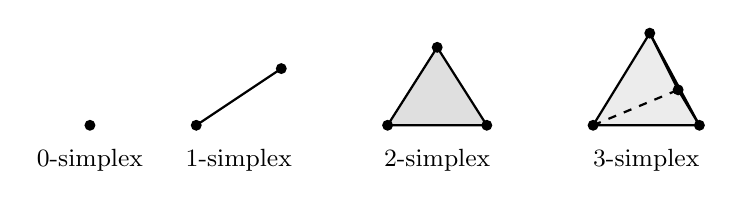
\begin{tikzpicture}[scale=0.9, v/.style={circle, fill=black, inner sep=1.4pt}]
  \node[v] at (0,0) {}; \node at (0,-0.5) {\small 0-simplex};
  \draw[thick] (1.5,0) node[v]{} -- (2.7,0.8) node[v]{}; \node at (2.1,-0.5) {\small 1-simplex};
  \fill[gray!25] (4.2,0) -- (5.6,0) -- (4.9,1.1) -- cycle;
  \draw[thick] (4.2,0) node[v]{} -- (5.6,0) node[v]{} -- (4.9,1.1) node[v]{} -- cycle; \node at (4.9,-0.5) {\small 2-simplex};
  \fill[gray!15] (7.1,0) -- (8.6,0) -- (7.9,1.3) -- cycle; \fill[gray!30] (8.6,0) -- (8.3,0.5) -- (7.9,1.3) -- cycle;
  \draw[thick] (7.1,0) node[v]{} -- (8.6,0) node[v]{} -- (7.9,1.3) node[v]{} -- cycle;
  \draw[thick] (8.6,0) -- (8.3,0.5) node[v]{} -- (7.9,1.3); \draw[thick, dashed] (7.1,0) -- (8.3,0.5);
  \node at (7.85,-0.5) {\small 3-simplex};
\end{tikzpicture}
\caption{Simplices of dimension 0 to 3.}\label{fig:simplices}
\end{figure}

\begin{definition}[Simplicial complex {\parencite{edelsbrunnerletscherzomorodian2002}}]
A \emph{simplicial complex} $K$ is a finite collection of simplices such that (i) every face of a simplex of $K$ is in $K$, and (ii) any two simplices of $K$ are disjoint or intersect in a common face.
Its \emph{vertex set} is the set of its 0-simplices.
\end{definition}

\begin{definition}[Abstract simplicial complex {\parencite{zomorodiancarlsson2005}}]
An \emph{abstract simplicial complex} on a vertex set $V$ is a collection $S$ of finite nonempty subsets of $V$ such that $\{v\} \in S$ for every $v \in V$, and $\tau \subseteq \sigma \in S$ implies $\tau \in S$.
A $k$-simplex is a set of $k+1$ vertices. Placing the vertices in general position gives a geometric realization $|S|$.
\end{definition}
The abstract version records only which vertices span simplices; it is the form in which nerves and Mapper graphs arise below.

\subsection{Skeleta and graphs}
\begin{definition}[Skeleton {\parencite{edelsbrunnerharerpatel2008}}]
The \emph{$k$-skeleton} $K^{(k)}$ of a simplicial complex $K$ is the subcomplex of all simplices of dimension at most $k$; the 0-skeleton is the vertex set.
\end{definition}
By the abstract definition, a finite graph $G = (V, E)$ \emph{is} a simplicial complex of dimension at most one: its vertices are 0-simplices and its edges are 1-simplices.
Its realization $|G|$, the graph viewed as a topological space, is a \emph{topological graph}.

\begin{example}\label{ex:graph}
Let $G$ have vertices $\{a,b,c,d\}$ and edges $\{a,b\}, \{b,c\}, \{a,c\}, \{c,d\}$, and let $K = G \cup \{\{a,b,c\}\}$ add the triangle on $a,b,c$.
Then $K^{(1)} = G$.
The graph $G$ has one loop, $a \to b \to c \to a$; in $K$ the triangle fills it.
A graph can therefore show a loop that the complex it came from does not have --- the situation of Section~\ref{sec:loops}.
\end{example}

\subsection{Nerves}
\begin{definition}[Nerve {\parencite{singh2007mapper,hatcher2001}}]
Let $\mathcal U = \{U_\alpha\}_{\alpha \in A}$ be a finite cover of a space $X$.
The \emph{nerve} $N(\mathcal U)$ is the abstract simplicial complex with vertex set $A$ in which a set $\{\alpha_0, \dots, \alpha_k\} \subseteq A$ spans a $k$-simplex if and only if $U_{\alpha_0} \cap \cdots \cap U_{\alpha_k} \neq \emptyset$.
\end{definition}

\begin{example}\label{ex:nerve}
Cover a circle by three arcs, each overlapping the next, with no point in all three.
The nerve has three vertices and three edges but no triangle: a hollow triangle, homotopy equivalent to the circle.
Cover a disk instead by three sets that share a common point: the nerve is a filled triangle, homotopy equivalent to a point, and so to the disk (Figure~\ref{fig:nerve}).
\end{example}

\begin{figure}[htbp]
\centering
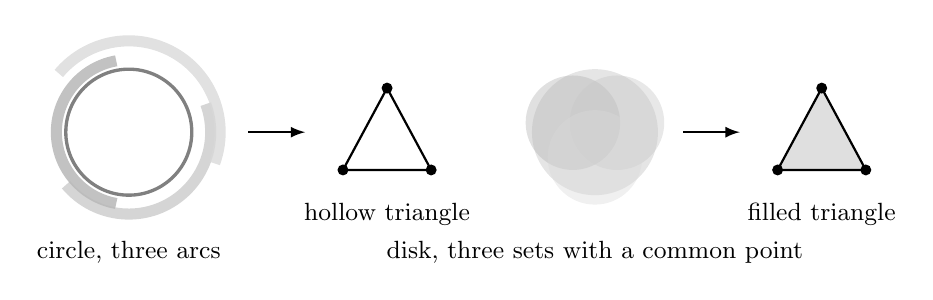
\begin{tikzpicture}[scale=0.8, v/.style={circle, fill=black, inner sep=1.4pt}]
  \draw[very thick, gray] (0,0) circle (1);
  \draw[line width=4pt, gray!80, opacity=0.6] (100:1.15) arc (100:260:1.15);
  \draw[line width=4pt, gray!55, opacity=0.6] (220:1.3) arc (220:380:1.3);
  \draw[line width=4pt, gray!30, opacity=0.8] (340:1.45) arc (340:500:1.45);
  \node at (0,-1.9) {\small circle, three arcs};
  \draw[-latex, thick] (1.9,0) -- (2.8,0);
  \draw[thick] (3.4,-0.6) node[v]{} -- (4.8,-0.6) node[v]{} -- (4.1,0.7) node[v]{} -- cycle;
  \node at (4.1,-1.3) {\small hollow triangle};
  \begin{scope}[xshift=7.4cm]
  \fill[gray!20] (0,0) circle (1);
  \fill[gray!60, opacity=0.4] (-0.35,0.15) circle (0.75); \fill[gray!45, opacity=0.4] (0.35,0.15) circle (0.75); \fill[gray!30, opacity=0.4] (0,-0.4) circle (0.75);
  \node at (0,-1.9) {\small disk, three sets with a common point};
  \draw[-latex, thick] (1.4,0) -- (2.3,0);
  \fill[gray!25] (2.9,-0.6) -- (4.3,-0.6) -- (3.6,0.7) -- cycle;
  \draw[thick] (2.9,-0.6) node[v]{} -- (4.3,-0.6) node[v]{} -- (3.6,0.7) node[v]{} -- cycle;
  \node at (3.6,-1.3) {\small filled triangle};
  \end{scope}
\end{tikzpicture}
\caption{Two covers and their nerves (Example~\ref{ex:nerve}).}\label{fig:nerve}
\end{figure}

\subsection{The nerve theorem}
In both examples the nerve has the shape of the space. The nerve theorem gives conditions under which this holds.
A set $C \subseteq \R^d$ is \emph{convex} if the segment between any two points of $C$ lies in $C$.

\begin{theorem}[Nerve theorem, closed convex version {\parencite[Thm.~3.9]{bauerkerberrollrolle2023}}]\label{thm:nerve}
If $X \subseteq \R^d$ is covered by finitely many closed convex sets $\mathcal C = \{C_1, \dots, C_n\}$, then $X \simeq |N(\mathcal C)|$.
\end{theorem}
An early closed-cover version is due to \textcite[Cor.~3]{borsuk1948}.
The idea behind the hypothesis is that a nonempty intersection of convex sets is convex, hence contractible, so each simplex of the nerve stands for a contractible piece of $X$.
There is also an open-cover version: if $\mathcal U$ is an open cover of a paracompact space $X$ and every nonempty finite intersection of its sets is contractible, then $X \simeq N(\mathcal U)$ \parencite{hatcher2001}.

\begin{remark}
Covers built from data are rarely this well behaved: the sets Mapper produces are clusters, not convex sets, and their intersections need not be contractible. A Mapper graph therefore need not have the shape of the underlying space, which is why Sections~\ref{sec:certify}--\ref{sec:shape} test its features rather than read them off.
\end{remark}

\subsection{Homology and Betti numbers}
\begin{definition}[Betti numbers {\parencite{hatcher2001}}]
The $k$-th \emph{Betti number} $b_k(X)$ is the rank of the $k$-th homology group $H_k(X)$. We use coefficients in $\Z_2$, so each $H_k$ is a vector space and $b_k$ is its dimension.
\end{definition}
The number $b_0$ counts path components \parencite{hatcher2001}, and $b_1$ counts independent loops.
For the complexes in this paper both are computable by linear algebra over $\Z_2$.
For a simplicial complex $K$, let $C_k$ be the $\Z_2$-vector space with basis the $k$-simplices, and let $\partial_k : C_k \to C_{k-1}$ send each simplex to the sum of its $(k-1)$-dimensional faces; then $H_k(K) = \ker \partial_k / \operatorname{im} \partial_{k+1}$.

For a finite graph $G$ with $V$ vertices, $E$ edges, and $C$ connected components, the Euler characteristic gives $V - E = b_0 - b_1$ with $b_0 = C$, so
\begin{equation}\label{eq:graph-b1}
  b_1(G) = E - V + C.
\end{equation}
In a complex of dimension two, triangles can fill loops, and
\begin{equation}\label{eq:complex-b1}
  b_1(K) = E - V + C - \rank \partial_2,
\end{equation}
where $\partial_2$ maps each triangle to its three edges.
A hollow triangle has $b_1 = 3 - 3 + 1 = 1$; filling it gives $\rank \partial_2 = 1$ and $b_1 = 0$.
Equation~\eqref{eq:complex-b1} is how Section~\ref{sec:loops} computes the loops of the full nerve.

\subsection{Reeb graphs and Reeb spaces}
\begin{definition}[Reeb graph {\parencite{carriereoudot2018,reeb1946}}]
Let $f : X \to \R$ be continuous. Write $x \sim y$ if $f(x) = f(y)$ and $x$ and $y$ lie in the same connected component of the level set $f^{-1}(f(x))$.
The \emph{Reeb graph} of $f$ is the quotient space $R_f(X) = X/{\sim}$.
\end{definition}
When $X$ is a smooth manifold and $f$ is a Morse function, or more generally of Morse type, $R_f(X)$ is a graph --- technically a multigraph --- and so a topological graph \parencite[p.~1334]{carriereoudot2018}.
For the height function on an upright torus, each level set collapses to one point per component: one point near the bottom and top, two in the middle band (Figure~\ref{fig:reeb}). The Reeb graph is a circle with two whiskers.
Replacing $\R$ by $\R^k$ and level sets by the preimages $f^{-1}(c)$, $c \in \R^k$, gives the \emph{Reeb space} \parencite{munchwang2016,edelsbrunnerharerpatel2008}.

\begin{figure}[htbp]
\centering
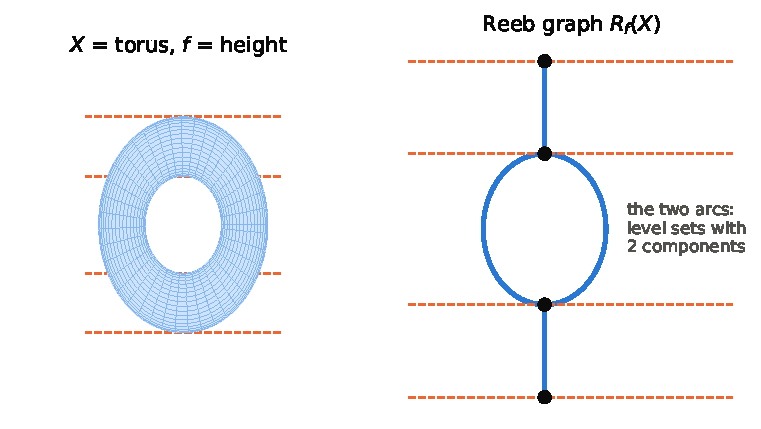
\includegraphics[width=0.62\textwidth]{reeb_torus.pdf}
\caption{The height function on a torus and its Reeb graph.}\label{fig:reeb}
\end{figure}

%======================================================================
\section{The Mapper algorithm}\label{sec:mapper}
%======================================================================
\subsection{Topological Mapper}
\begin{definition}[Mapper {\parencite{singh2007mapper,deymemoliwang2017}}]
Let $f : X \to Z$ be continuous and let $\mathcal U = \{U_\alpha\}$ be a finite open cover of $Z$.
Split each preimage $f^{-1}(U_\alpha)$ into its path components; together they form the \emph{pullback cover} $f^*\mathcal U$ of $X$.
The \emph{Mapper} is its nerve, $M(\mathcal U, f) = N(f^*\mathcal U)$.
\end{definition}
For $Z = \R$, Mapper is a discrete estimator of the Reeb graph; for $Z = \R^d$ it approximates the Reeb space \parencite{carrieremicheloudot2018,munchwang2016}.
Its loops are controlled by those of $X$:

\begin{theorem}[Dey--M\'emoli--Wang {\parencite{deymemoliwang2017}}]\label{thm:dmw}
If $\mathcal U$ is a path-connected cover of a compact space $X$, the nerve map induces a surjection $H_1(X) \to H_1(N(\mathcal U))$, with $\Z_2$ coefficients.
\end{theorem}
Mapper's pullback cover consists of path components, so it is path-connected, and therefore
\begin{equation}\label{eq:mapper-b1}
  b_1(M(\mathcal U, f)) \le b_1(X).
\end{equation}
This bound concerns the nerve, a simplicial complex. Software outputs only its 1-skeleton, whose loops are not bounded this way (Example~\ref{ex:graph}); Section~\ref{sec:loops} shows the difference in our data.

\subsection{Statistical Mapper}
A \emph{point cloud} is a finite set $P \subseteq \R^n$ with Euclidean distance.
In the statistical version of Mapper, clustering plays the role of path components: each preimage $f^{-1}(U_\alpha) \cap P$ is split into clusters \parencite{singh2007mapper}.
The algorithm has four steps:
\begin{enumerate}
  \item choose a \emph{lens} $f : P \to \R^k$;
  \item cover $f(P)$ by overlapping sets;
  \item cluster each preimage, in the full space $\R^n$;
  \item form the \emph{Mapper graph}: one vertex per cluster, and one edge for each pair of clusters that share a point.
\end{enumerate}
Steps 1--3 build a cover of $P$ and step 4 takes its nerve \parencite{singh2007mapper}, keeping only the 1-skeleton.
The lens decides which points are clustered together; the clustering itself uses all $n$ coordinates.

\begin{example}\label{ex:toy}
Take 240 noisy points on a circle, the lens $f(x,y) = y$, and five intervals with 30\% overlap.
DBSCAN (Section~\ref{sec:dbscan}) splits the five preimages into $1, 2, 2, 2, 1$ arcs, and arcs in overlapping intervals share points.
The graph is a single loop, $b_1 = 8 - 8 + 1 = 1$: the shape of the circle, and its Reeb graph for the height function (Figure~\ref{fig:toy}).
\end{example}

\begin{figure}[htbp]
\centering
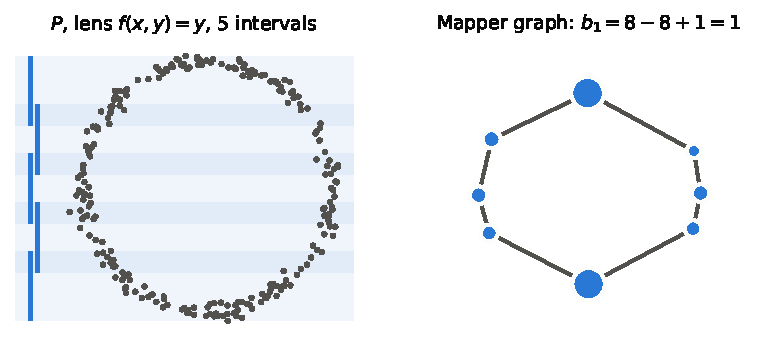
\includegraphics[width=0.75\textwidth]{toy_mapper.pdf}
\caption{Mapper on a noisy circle (Example~\ref{ex:toy}).}\label{fig:toy}
\end{figure}

\subsection{The lens: principal component analysis}
Among the Mapper applications reviewed by \textcite{madukpe2026review}, principal component analysis (PCA) is the most commonly used lens; we use a two-dimensional PCA lens.
PCA finds new uncorrelated variables, linear combinations of the old ones, that successively capture as much variance as possible \parencite{jolliffecadima2016,pearson1901}.

Let the data be $m$ observations of $n$ features, and subtract each column's mean to obtain the centered matrix $\mathbf A \in \R^{m \times n}$.
Centering is not a choice that changes the answer: variance is measured around the mean, so it changes neither the covariance matrix nor the principal components, and it makes $(m-1) S = \mathbf A^{\mathsf T} \mathbf A$, which turns PCA into a statement about $\mathbf A$ itself \parencite{jolliffecadima2016}.
Here $S = \frac{1}{m-1}\mathbf A^{\mathsf T}\mathbf A$ is the covariance matrix: its diagonal entries are the feature variances and its off-diagonal entries the covariances.

$S$ is positive semidefinite, since $x^{\mathsf T} S x = \frac{1}{m-1}\|\mathbf A x\|^2 \ge 0$ for every $x \in \R^n$, so it has real, nonnegative eigenvalues and an orthonormal basis of eigenvectors. The variance of the data along a unit vector $v$ is $v^{\mathsf T} S v$, which is maximized by a top eigenvector.

\begin{theorem}[Singular value decomposition {\parencite{axler2024ladr}}]
Let $\mathbf A$ have rank $r \ge 1$. Then $\mathbf A = \mathbf U \boldsymbol\Sigma \mathbf V^{\mathsf T}$, where $\mathbf U \in \R^{m \times r}$ and $\mathbf V \in \R^{n \times r}$ have orthonormal columns and $\boldsymbol\Sigma = \operatorname{diag}(\sigma_1 \ge \cdots \ge \sigma_r > 0)$.
\end{theorem}
The columns of $\mathbf V$ are eigenvectors of $\mathbf A^{\mathsf T}\mathbf A$, and the columns of $\mathbf U$ eigenvectors of $\mathbf A\mathbf A^{\mathsf T}$, for the nonzero eigenvalues $\sigma_i^2$; hence the eigenvalues of $S$ are $\lambda_i = \sigma_i^2/(m-1)$ and the principal directions are the columns $v_i$ of $\mathbf V$ \parencite{jolliffecadima2016}.
Keeping the first $k$ directions, $\mathbf V_k = [v_1 \cdots v_k]$, the lens is $f(x) = \mathbf V_k^{\mathsf T} x$ and the score matrix is $\mathbf Z_k = \mathbf A \mathbf V_k = \mathbf U_k \boldsymbol\Sigma_k$.
The matrix $\mathbf A_k = \mathbf U_k \boldsymbol\Sigma_k \mathbf V_k^{\mathsf T}$ is the closest matrix of rank at most $k$ to $\mathbf A$, both in the operator norm, with error $\sigma_{k+1}$ \parencite{axler2024ladr}, and in the least-squares sense \parencite{jolliffecadima2016}.
The proportion of variance explained by component $j$ is $\lambda_j / \sum_l \lambda_l = \sigma_j^2 / \sum_l \sigma_l^2$ \parencite{jolliffecadima2016}.

We take $k = 2$. On our data the first two components explain \PCone\% and \PCtwo\% of the variance.
The cover lives in $\R^k$: with ten intervals per axis, $k = 2$ gives 100 cubes, while $k = 3$ would give 1{,}000, most of them nearly empty; and a two-dimensional lens can be drawn and read.
Because PCA is linear it can flatten curved structure; this is acceptable here because clustering happens in the full space, and Section~\ref{sec:certify} repeats the stability analysis with three other lenses, including the nonlinear Isomap \parencite{tenenbaum2000isomap}.

\subsection{The cover}
The image $f(P) \subseteq \R^k$ is covered by overlapping hypercubes: each axis is cut into intervals that overlap their neighbors by a fixed percentage \parencite{singh2007mapper,madukpe2026review}.
Two parameters set the resolution, the number of intervals and the percentage overlap \parencite{singh2007mapper}, and the resulting graph depends on them; tuning them on real data is not easy \parencite{carrieremicheloudot2018}.
We use ten intervals per axis with 30\% overlap and test the results over a grid of alternatives (Section~\ref{sec:certify}).

\subsection{Clustering: DBSCAN}\label{sec:dbscan}
Each preimage is clustered with DBSCAN, the second most common choice in reviewed Mapper applications after hierarchical clustering \parencite{madukpe2026review}.
It needs no preset number of clusters, finds clusters of arbitrary shape, and labels isolated points as noise \parencite{ester1996dbscan}.
Fix a point cloud $P$ with distance $d$, a radius $\varepsilon > 0$, and a count $M \in \N$ (called Eps and MinPts by \textcite{ester1996dbscan}). The following definitions are theirs.

\begin{definition}
The \emph{$\varepsilon$-neighborhood} of $p \in P$ is $N_\varepsilon(p) = \{ q \in P : d(p,q) \le \varepsilon \}$, and $p$ is a \emph{core point} if $|N_\varepsilon(p)| \ge M$.
A point $p$ is \emph{directly density-reachable} from $q$ if $p \in N_\varepsilon(q)$ and $q$ is a core point, and \emph{density-reachable} from $q$ if there is a chain $q = p_1, p_2, \dots, p_k = p$ in which each $p_{i+1}$ is directly density-reachable from $p_i$.
Points $p$ and $q$ are \emph{density-connected} if both are density-reachable from some common point $o$.
\end{definition}
\begin{definition}
A \emph{cluster} is a nonempty $C \subseteq P$ such that (i) if $p \in C$ and $q$ is density-reachable from $p$, then $q \in C$ (maximality), and (ii) any two points of $C$ are density-connected (connectivity).
\emph{Noise} is the set of points of $P$ in no cluster; it depends on the chosen $(\varepsilon, M)$.
\end{definition}
\begin{lemma}[{\textcite{ester1996dbscan}}]
If $C$ is a cluster and $p \in C$ is a core point, then $C = \{ o \in P : o \text{ is density-reachable from } p \}$.
\end{lemma}
The lemma is why the algorithm is correct: a cluster is determined by any one of its core points, so starting from an unclassified core point and collecting everything density-reachable from it recovers exactly its cluster. The algorithm loops over the points and expands a new cluster from each unclassified core point \parencite[p.~229]{ester1996dbscan}; a point that is not a core point is marked noise for now, and a border point first marked noise is relabeled if a later cluster reaches it.
\textcite{ester1996dbscan} allow different parameters $(\varepsilon_i, M_i)$ for each cluster; the algorithm, and our analysis, use one global pair, $\varepsilon = 1.0$ in standardized units and $M = 4$.
Figure~\ref{fig:dbscan} shows the three kinds of point.

\begin{figure}[htbp]
\centering
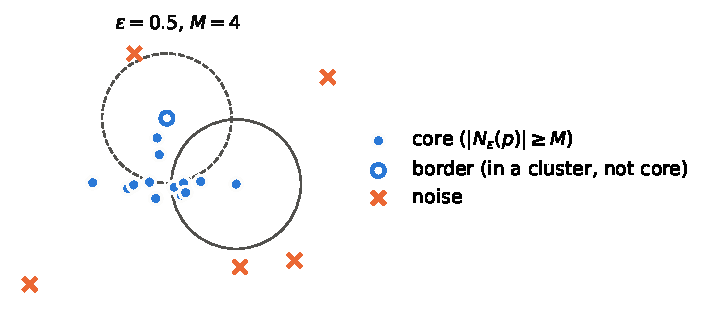
\includegraphics[width=0.6\textwidth]{dbscan_toy.pdf}
\caption{Core, border, and noise points for $\varepsilon = 0.5$, $M = 4$. Solid circle: a core point's $\varepsilon$-ball holds six points. Dashed circle: a border point's ball holds three, including a core point, so it joins the cluster. Crosses: noise, each more than $\varepsilon$ from every core point.}\label{fig:dbscan}
\end{figure}

\subsection{The graph and its implementation}
Each cluster becomes a vertex, and two clusters are joined by an edge when they share at least one point, which happens because neighboring cubes overlap \parencite{singh2007mapper}.
The clusters form a cover of the non-noise part of $P$, and the graph is the 1-skeleton of its nerve: three clusters with a common point span a triangle in the nerve, but the graph keeps only the three edges.
We use KeplerMapper, a Python implementation that works with scikit-learn-compatible clustering and scaling algorithms \parencite{vanveen2019keplermapper,pedregosa2011sklearn}, developed under the scikit-tda project \parencite{keplermapper_repo}.

%======================================================================
\section{Related work}\label{sec:related}
%======================================================================
\subsection{How pitches are labeled and grouped}
MLB's pitch labels come from a patented classifier.
In the patent, a pitch is classified from its measured properties --- break, speed, direction of movement --- together with the pitch types previously determined to be in that pitcher's repertoire, and is assigned the type most likely to match its trajectory \parencite{paul2014patent}.
MLB describes the system as patented neural-network software, customized for every pitcher, that classifies nearly 750{,}000 pitches a season \parencite{sharpe2020classification}.
The labels are therefore names within each pitcher's arsenal rather than regions of a common space, which is one reason the same physical shape can carry different labels for different pitchers.

Unsupervised work groups pitches by their physics.
\textcite{pane2013trouble} classify PITCHf/x pitches by model-based clustering with a multivariate Gaussian mixture.
\textcite{camp2020clustering} apply $k$-means to the movement, velocity, and spin rate of 2016--17 Statcast pitches and find 30 subtypes within the nine prominent Statcast pitch types for each handedness; these clusters subdivide the existing labels rather than test them.
Closest to this paper, \textcite{maloof2026classify} apply persistent homology to a smoothed density of 4.47 million NCAA Division I pitches, in speed relative to the pitcher's fastest pitch, horizontal break, and induced vertical break.
They find three dominant density peaks --- fastball, breaking ball, and changeup --- draw the boundaries between them by watershed segmentation, and, combining persistent homology with curvature and spectral-graph analyses, conclude that finer pitch names are locations along continuous ridges.
Their article is not peer-reviewed.
We reach a compatible picture by a different route: Major League data, nine features including spin and release, one point per pitcher and pitch type, the Mapper graph and the homology of its nerve, Vietoris--Rips persistence (which detects gaps rather than modes), and null models; and we replicate their density-peak analysis on our data (Section~\ref{sec:certify}).

\subsection{Topological data analysis in sports}
\textcite{lum2013extracting} built a topological network from NBA player statistics --- a Reeb-graph-based construction with the same inputs as Mapper (a filter, a resolution, and an overlap) --- and found 13 player positions in place of the traditional five.
Persistent homology has been applied to NHL team composition \parencite{goldfarb2014hockey} and, through lower-star filtrations of player networks, to predicting ATP tennis matches \parencite{schwaderer2026tennis}.
\textcite{madukpe2026review} survey Mapper applications from 2007 to 2025.

\subsection{Validating Mapper}
Mapper's output depends strongly on the cover parameters \parencite{carrieremicheloudot2018}.
\textcite{carrieremicheloudot2018} develop a statistical analysis and a principled parameter selection for Mapper; we use a parameter grid and resampling instead, and their approach is an alternative.
\textcite{vejdemojohansson2018certified} note that Mapper does not check whether its cover meets the requirements of the nerve lemma, and propose statistical tests for obstructions.
\textcite{topaz2026null} show that the covariance structure of data alone can make Mapper communities look differentiated, propose a Gaussian null model with the sample covariance, and find that four published Mapper analyses do not exceed it at the 0.05 level once singleton communities are set aside; as Topaz notes, a non-rejection does not rule out subtypes.
We arrived at the same covariance-matched null independently, designing our comparisons in the spirit of hypothesis testing for persistent homology \parencite{robinsonturner2017,blumberg2014}, and apply it beyond communities: to the graph's features, its loops, the homology of the point cloud, its intrinsic dimension, and its density peaks.

%======================================================================
\section{Data}\label{sec:data}
%======================================================================
We use Statcast pitch-tracking data \parencite{savantcsvdocs}, downloaded with pybaseball \parencite{ledoux_pybaseball}.
The main analysis uses the 2025 regular season and postseason, \NPitches{} pitches.
Each pitch is described by nine features: release speed; horizontal and vertical movement $pfx_x$ and $pfx_z$ (in feet, from the catcher's view); spin rate; spin axis; extension; and the horizontal and vertical release position \parencite{savantcsvdocs}.
Statcast documents $pfx_z$ only as vertical movement; that it excludes gravity, so that it is induced vertical break, is our inference from the data (four-seam fastballs average about $+1$ foot).

Left-handed pitchers are mirrored into the right-handed frame: $pfx_x$ and the horizontal release position change sign, and the spin axis $\theta$ becomes $360^\circ - \theta$.
The spin axis is an angle, so $\theta$ and $\theta + 360^\circ$ are the same direction; we encode it as the point $(\cos\theta, \sin\theta)$ on the circle rather than as a number in $[0, 360)$, giving nine coordinates in all with the axis counting as two.
Each pitch also carries a Statcast pitch-type code \parencite{mlbglossary_pitchtypes}.

The unit of analysis is a \emph{pitch shape}: the average of one pitcher's pitches of one type.
This removes pitch-to-pitch noise and keeps each pitcher's stable profile, and gives \NShapes{} shapes in $\R^{\NFeatures}$, standardized to mean zero and unit variance.
No minimum pitch count was applied in the fit. The median shape averages \MedianPitches{} pitches, but \PctLtFive\% average fewer than five and \PctLtTwenty\% fewer than twenty; the \NSlow{} slow shapes (below 70 mph) are thinnest, with a median of \SlowMedian{} pitches and a quarter at \SlowQ{} or fewer.
Table~\ref{tab:thin} repeats the main Mapper fit with minimum counts of 10 and 20.
Statcast revises some pitch labels after the fact, so rebuilding the shapes from a later download gives counts that differ by a few (\SSOneShapes{} rather than \NShapes).

\begin{table}[htbp]
\centering
\begin{tabular}{rrrrcc}
\toprule
Minimum pitches & Shapes & Slow shapes & Components & Slow shapes isolated & Velocity ordering $\rho$ \\
\midrule
1 & \SSOneShapes & \SSOneSlow & \SSOneComp & \SSOneIso & \SSOneRho \\
10 & \SSTenShapes & \SSTenSlow & \SSTenComp & \SSTenIso & \SSTenRho \\
20 & \SSTwentyShapes & \SSTwentySlow & \SSTwentyComp & \SSTwentyIso & \SSTwentyRho \\
\bottomrule
\end{tabular}
\caption{The main Mapper fit with a minimum pitch count per shape. The velocity ordering is unaffected; slow shapes stay off the continuum, but at a minimum of 20 they are too few to form clusters of their own.}\label{tab:thin}
\end{table}

Three more seasons are used in Section~\ref{sec:consequences}: 2026 (\NPitchesTwentySix{} pitches) to replicate the evaluation results out of sample, and 2023 (\NPitchesTwentyThree) and 2024 (\NPitchesTwentyFour) for the year-over-year development tests.

%======================================================================
\section{Certifying the Mapper picture}\label{sec:certify}
%======================================================================
A Mapper graph is a picture, not a test.
For each feature it shows we ask two questions: does the feature survive reasonable changes to the construction, and does a null model without the structure in question reproduce it?
We then compute invariants that do not depend on Mapper's parameters: the homology of the full nerve, persistent homology, intrinsic dimension, and density peaks.

\subsection{Stability}
We refit the graph over a 27-point grid --- 8, 10, or 12 intervals per axis, 20, 30, or 40\% overlap, and $\varepsilon = 0.8$, 1.0, or 1.2 --- and 30 times on a random 80\% of pitchers drawn without replacement.
Every fit is repeated with four lenses: the PCA lens; velocity against induced vertical break; a two-dimensional Isomap embedding; and a one-dimensional density lens, the mean distance to the ten nearest neighbors.
Node labels change between fits, so features are defined by content:
\begin{itemize}
  \item \emph{connectivity}: the number of components and the size of the largest;
  \item \emph{slow-pitch isolation}: whether most shapes slower than 70 mph lie outside the largest component;
  \item \emph{velocity ordering}: Spearman's $\rho$ between node velocity and position along the shortest path from the most-curveball node to the most-four-seam node, counted as present when $\rho \ge 0.7$.
\end{itemize}

\subsection{Null models}
Each null is refit through the identical pipeline:
\begin{itemize}
  \item a \emph{Gaussian null} with the same mean and covariance as the shapes, which has no structure beyond its second moments;
  \item a \emph{within-type shuffle}, in which each feature is permuted independently among shapes of the same pitch type, keeping each type's marginal distributions but destroying the joint structure inside it;
  \item a \emph{spin-pair shuffle}, the same but permuting $(\cos\theta, \sin\theta)$ together, so that shuffled shapes still have a valid spin axis.
\end{itemize}
A feature counts as evidence of structure only if real fits show it clearly more often than null fits.

\subsection{Loops of the full nerve}
For each fit we compute the first Betti number of the graph by~\eqref{eq:graph-b1} and of the full nerve by~\eqref{eq:complex-b1}, adding a triangle for every three clusters with a common point and computing $\rank \partial_2$ over $\Z_2$.
By~\eqref{eq:mapper-b1}, loops of the nerve that a null model also produces are not evidence of loops in the data.

\subsection{Persistent homology}
For a finite metric space $(P, d)$ and scale $t \in \R$, the Vietoris--Rips complex is $\mathrm{Rips}_t(P) = \{ \emptyset \neq S \subseteq P : \diam S \le t \}$ \parencite{bauer2021ripser}.
As $t$ grows these complexes are nested, and persistent homology records the scale at which each component or loop is born and dies \parencite{edelsbrunnerletscherzomorodian2002,zomorodiancarlsson2005}.
We compute it with Ripser \parencite{bauer2021ripser,tralie2018ripserpy} on five random subsamples of 1{,}000 standardized shapes, for the real data and the nulls.
Following the usual reading of persistence diagrams, points far from the diagonal are features and points near it are noise \parencite{fasy2014confidence}; we do not compute formal confidence sets, but compare with the nulls, counting an $H_0$ bar as long-lived if it dies after three times the median $H_0$ death and an $H_1$ loop as real if its persistence exceeds twice that.
An $H_0$ bar that lives long is a gap between groups of shapes; an $H_1$ bar is a loop.

\subsection{Intrinsic dimension}
We estimate the dimension of the point cloud with the maximum-likelihood estimator of \textcite{levinabickel2004}, using ten neighbors and the averaging of \textcite{mackay2005comments}, and with TwoNN \parencite{facco2017twonn}.
Both use nearest-neighbor distances. The comparison is with the spin-pair shuffle, which keeps each type's marginals and the spin-axis constraint, and is made overall and within each pitch type.

\subsection{Density peaks}
Vietoris--Rips persistence detects gaps; it cannot tell a space with one dense region from one with several.
Following \textcite{maloof2026classify}, we compute the persistence of the superlevel sets of a smoothed density, at the pitch level: speed relative to the pitcher's 95th-percentile speed in that game, horizontal break, and induced vertical break, on a $50^3$ grid (horizontal and vertical break from $-25$ to 25 inches, relative speed from $-25$ to 5 mph), smoothed by a Gaussian of one grid cell.
Each peak's persistence is compared with the largest secondary peak in 50 covariance-matched Gaussian replicates, giving a Monte Carlo $p$-value.
A Gaussian has one peak, so this test only shows that there is more than one; small peaks are judged by their robustness to the smoothing (1, 1.5, and 2 cells) and to random halves of the data.
We repeat the analysis in one dimension, for the pitch shapes along the first principal component.

%======================================================================
\section{The shape of pitch space}\label{sec:shape}
%======================================================================
\plan{Lens figure (PC1 \PCone\%, PC2 \PCtwo\%); Mapper graph (\NNodes{} nodes, \NEdges{} edges, \NComponents{} components); stability table; nulls reproduce the velocity ordering in every fit and slow-pitch isolation in 50--78\% of fits.}

\subsection{Loops are artifacts of the 1-skeleton}\label{sec:loops}
\plan{Graph $b_1 = E - V + C = \GraphBone$; full nerve $b_1 = \NerveBone$ ($\rank_{\Z_2}\partial_2$); across the grid, graph $b_1$ \GridGraphBoneMin--\GridGraphBoneMax{} vs.\ nerve \GridNerveBoneMin--\GridNerveBoneMax, in the range of the nulls. Persistent homology: no persistent $H_1$. Figure \texttt{nerve\_b1}.}

\subsection{Connected, about six-dimensional, and multimodal}
\plan{Intrinsic dimension \DimMLE{} (TwoNN \DimTwoNN) vs.\ fair null \DimNullMLE.
Density peaks: three robust (fastball; breaking ball, relative persistence \PeakBB; changeup, \PeakCH), a small stable curveball bump, a fragile sweeper bump; locations within a few inches of Maloof et al.'s college peaks. Labels beyond the three classes sit on ridges.
Source: DISCOVERY\_FINDINGS ``Density peaks''.}

%======================================================================
\section{Consequences for evaluation and development}\label{sec:consequences}
%======================================================================
\subsection{Grading within a label is fragile near boundaries}
\plan{Boundary pitches (nearest other-pitcher shapes in flight space, velocity relative to the pitcher's fastest pitch): \LSTwentyFiveBoundary{} of \LSTwentyFiveEligible{} (\LSTwentyFiveBoundaryPct\%) in 2025; \LSTwentySixBoundary{} of \LSTwentySixEligible{} in 2026.
Median grade shift \LSTwentyFiveShift{} (2026: \LSTwentySixShift); $\ge$ 1 SD for \LSTwentyFiveOneSDPct\% (\LSTwentySixOneSDPct\%); shift $>$ 2 SE for \LSTwentyFiveTwoSEPct\% (\LSTwentySixTwoSEPct\%); crosses average for \LSTwentyFiveCrossPct\% (\LSTwentySixCrossPct\%).
Model-free: actual SwStr\% percentile moves a median \LSTwentyFivePctChange{} points (2026: \LSTwentySixPctChange).
Scope: grading \emph{within} a label; FanGraphs' Stuff+ is on one common scale \parencite{mcgrattan2023stuffplus}.
Two confounds fixed and reported: same-pitcher delivery; absolute velocity.}

\subsection{Moving toward better neighbors}
\plan{Pre-specified design (committed before running): progress toward the better-scoring third of a pitch's 20 nearest other-pitcher shapes vs.\ change in actual SwStr\%, chase\%, xwOBA on contact; placebos toward a random and the worst third; primary pairs 2024$\to$2025 and 2025$\to$2026 (\DevN{} pitches). Result: hypothesis not supported, $\beta = \DevBetterBeta$ pp per full move (CI \DevBetterLo{} to \DevBetterHi, $p = \DevBetterP$); placebos random \DevRandomBeta{} ($p = \DevRandomP$) and worst \DevWorseBeta{} ($p = \DevWorseP$), so the pre-specified failure criterion is met. Exploratory joint model (labeled as such): toward the neighborhood \DevExRandomBeta{} ($p = \DevExRandomP$), toward its better part beyond that \DevExBetterBeta{} ($p = \DevExBetterP$) --- a distinctiveness hypothesis for future work.}

\subsection{Distinctiveness}
\plan{Pre-specified typicality test (\texttt{src/stuffplus/typicality.py}): typicality = $-\log$ mean distance to the 20 nearest other-pitcher shapes; actual SwStr\% on typicality, controlling for the physics-only model's prediction. Primary 2025--26 (control out-of-sample): $\beta = \TypBeta$ pp per SD (CI \TypLo{} to \TypHi), robust to $K$; harder contact too; secondary 2023--24 weaker ($\TypSecBeta$, $p = \TypSecP$), as expected with an in-sample control. Caveat: typicality may proxy model misfit.}

\subsection{A development planner}
\plan{Profile held fixed (arm angle, extension; velocity and spin bands). Value $V = \gamma\,\hat p_{\text{miss}} + \beta\,\text{typ}$, both coefficients from the pre-specified typicality model. Steps on a $k$-nearest-neighbor graph of real shapes; velocity and spin weighted as arm talent; season budget from observed one-season changes; destination = best value within three seasons; benchmarks = milestones along that one path; value checked monotone.
Young-arm search (2026, age $\le 25$): \YoungPlanned{} pitches planned, \YoungClear{} clear cases; illustrated by Gage Jump's slider (age \JumpAge, \JumpN{} pitches): glove-side sweep \JumpSweepStart{} $\to$ \JumpSweepOne{} in (season 1, $+\JumpGainOne$ pp) $\to$ \JumpSweepEnd{} in (season \JumpEndSeason, $+\JumpGainEnd$ pp), a pure shape plan. Figure \texttt{development\_path}. Illustrative, not validated; the earlier Eovaldi neighborhood (figure \texttt{pitch\_design}) moves to an appendix or is dropped.
Connection to the topology: connectedness guarantees a path exists; shortest paths on a nearest-neighbor graph are how Isomap approximates geodesic distances \parencite{sklearn_userguide_manifold}, a method due to \textcite{tenenbaum2000isomap}.}

%======================================================================
\section{Limitations}\label{sec:limits}
%======================================================================
\plan{One fitting season (2026 replication for the evaluation result only); no minimum pitch count in the fit; persistent homology and intrinsic dimension not rerun with a minimum count; no formal confidence band on persistence diagrams; Mapper parameters by grid, not a principled method; our Stuff+-style model is a reimplementation; development result observational.}

%======================================================================
\section{Conclusion}\label{sec:conclusion}
%======================================================================
\plan{Mapper gives the picture; homology, nulls, dimension, and density certify it. Pitch labels are conventions on a connected, three-peaked space, which matters for how pitches are graded and compared. Future work: movement relative to arm slot; other seasons and levels; principled parameter choice.}

\appendix
\section{Parameters and reproducibility}
\plan{All parameters; code at \url{https://github.com/WillPaz16/tda-pitch-clustering}; every number generated by \texttt{src/viz/paper\_numbers.py}; seeds.}

\section{Use of AI assistance}
\plan{Adapt the README disclosure: what Claude did, what was verified and how (citation ledger, blind checks, page-image reads), and what the author checked.}

\printbibliography

\end{document}
